\section{实验原理与方法}

本文所用的实验项目、样品与测试条件汇总于表\ref{tab:projects}。两条制备路线均以钛酸四丁酯为前驱体，产物在相同温度序列下热处理，以保证后续比较的可比性。

\begin{figure*}[htbp]
  \centering
  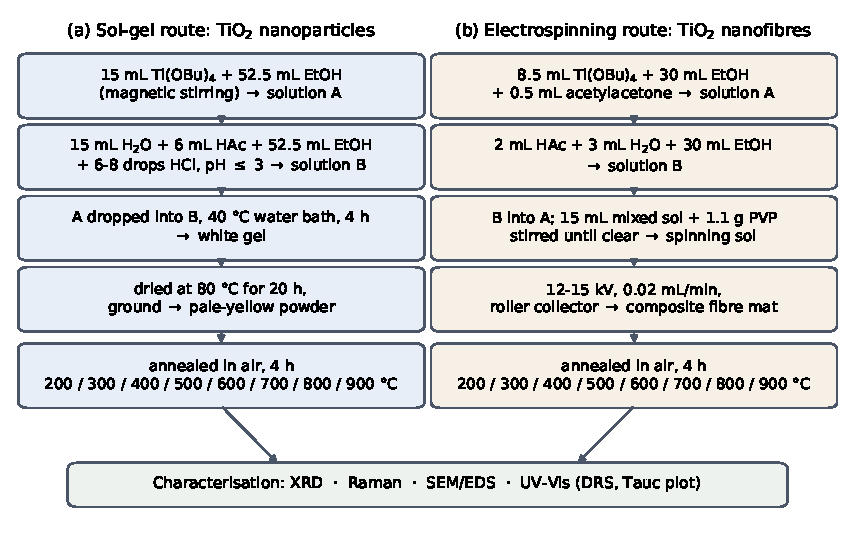
\includegraphics[width=0.86\textwidth]{figures/fig1_flow.pdf}
  \caption{溶胶-凝胶法 (a) 与静电纺丝法 (b) 的制备流程及后续表征示意}
  \label{fig:flow}
\end{figure*}

\begin{table}[htbp]
  \centering
  \caption{本文分析的实验项目与主要测试条件}
  \label{tab:projects}
  \footnotesize
  \begin{tabular}{@{}>{\raggedright\arraybackslash}p{2.05cm}>{\raggedright\arraybackslash}p{2.85cm}>{\raggedright\arraybackslash}p{1.9cm}@{}}
    \toprule
    实验项目 & 主要仪器/条件 & 数据来源 \\
    \midrule
    溶胶-凝胶制备 & 恒温水浴、马弗炉，200—900 $^\circ$C/4 h & 本文实验记录 \\
    静电纺丝制备 & PS-ZJ03 纺丝机，12—15 kV & 本文实验记录 \\
    X 射线衍射 & Cu $K\alpha$，20$^\circ$—80$^\circ$ & 第六组等 \\
    扫描电镜与能谱 & S-4800，10 kV，SE(U) & 第五组 \\
    拉曼光谱 & 633 nm 激发，50—1000 cm$^{-1}$ & 九组谱库 \\
    紫外-可见漫反射 & U-3900，300—600 nm & 第四组 \\
    \bottomrule
  \end{tabular}
\end{table}

\subsection{溶胶-凝胶法制备 TiO$_2$ 纳米颗粒}

溶胶-凝胶法的实质是金属醇盐的水解与缩聚：Ti(OBu)$_4$ 先与水反应生成羟基衍生物 Ti—OH，随后两个羟基（或羟基与残留烷氧基）缩合形成 Ti—O—Ti 桥键，逐渐构筑三维网络\cite{li2008制备}。体系中的冰醋酸既作为抑制剂与中心离子配位、降低水解速率，又通过调节 pH 使胶粒表面带同种电荷而避免团聚；盐酸将 pH 控制在 3 以下，进一步抑制过快水解，从而获得澄清、稳定的溶胶。溶胶在 40 $^\circ$C 水浴中经 4 h 交联老化形成白色凝胶，80 $^\circ$C 干燥 20 h 排出自由水与部分有机物，研磨后得到淡黄色干凝胶粉末，最后在空气气氛中于设定温度保温 4 h，完成有机残留的烧除与晶化。

具体配比与流程见图\ref{fig:flow}(a)：15 mL 钛酸四丁酯缓慢滴入 52.5 mL 无水乙醇得到溶液 A；15 mL 去离子水、6 mL 冰醋酸与 52.5 mL 无水乙醇混合后滴加 6—8 滴浓盐酸得到溶液 B；将 A 缓慢滴入 B 后于 40 $^\circ$C 反应 4 h。

\begin{table}[htbp]
  \centering
  \caption{溶胶-凝胶法制备 TiO$_2$ 的实验变量与预期结果}
  \label{tab:sg}
  \footnotesize
  \begin{tabular}{@{}p{2.4cm}p{4.1cm}@{}}
    \toprule
    实验变量 & 预期实验现象与结果 \\
    \midrule
    水量与酸量（pH） & 水量增大、pH 升高时水解加快，易生成沉淀；pH$\,\leq\,$3 时溶胶透明稳定 \\
    滴加顺序与速率 & A 滴入 B 且缓慢滴加时成胶均匀；滴加过快易局部水解产生颗粒团聚 \\
    水解温度 & 40 $^\circ$C 时缩聚速率适中；温度过高则凝胶时间缩短、孔径分布变宽 \\
    干燥条件 & 80 $^\circ$C 保温 20 h 可避免残存溶剂在煅烧时造成开裂 \\
    热处理温度 & 200—600 $^\circ$C 保持锐钛矿；700 $^\circ$C 起出现金红石；晶粒随温度长大 \\
    \bottomrule
  \end{tabular}
\end{table}

操作中需注意三点：其一，A 液滴入 B 液时必须缓慢并保持剧烈搅拌，防止局部浓度过高形成沉淀；其二，体系对水敏感，所用玻璃器皿需充分干燥；其三，干燥不充分的凝胶在高温煅烧时因溶剂急剧汽化而开裂，会破坏颗粒的均匀性。

\subsection{静电纺丝法制备 TiO$_2$ 纳米纤维}

静电纺丝利用高压静电场对聚合物溶液的作用实现纤维成型：液滴在针头处带电后同时受到外电场库仑力与表面电荷间的静电斥力，被拉伸成锥形（泰勒锥）；当电场强度超过临界值时，射流从锥顶喷出，在飞行过程中经历拉伸、鞭动、溶剂挥发与固化，最终以无纺布形式沉积在收集极上\cite{zhao2019静电纺丝}。本文以 PVP（$M\approx1.3\times10^{6}$）作为增稠与纺丝模板组分，它赋予溶胶足够的粘弹性以保证射流连续，并在后续煅烧中被完全烧除，留下 TiO$_2$ 纤维。

前驱体溶胶的配制见图\ref{fig:flow}(b)：8.5 mL 钛酸四丁酯与 0.5 mL 乙酰丙酮依次加入 30 mL 无水乙醇得到 A；2 mL 冰乙酸、3 mL 去离子水与 30 mL 无水乙醇混合得到 B；B 缓滴入 A 后取 15 mL 混合液加入 1.1 g PVP，室温搅拌至完全溶解且无气泡。纺丝时推进速率设为 0.02 mL/min，电压 12—15 kV，以滚筒为收集极。

\begin{table}[htbp]
  \centering
  \caption{静电纺丝法制备 TiO$_2$ 纤维的实验变量与预期结果}
  \label{tab:es}
  \footnotesize
  \begin{tabular}{@{}p{2.4cm}p{4.1cm}@{}}
    \toprule
    实验变量 & 预期实验现象与结果 \\
    \midrule
    PVP 含量 & PVP 过少时粘度过低、易形成液滴或珠粒；过多则纤维直径增大甚至堵塞针头 \\
    纺丝电压 & 低于临界电压时无法克服表面张力，无射流；过高则射流不稳定、纤维直径离散度增大 \\
    推进速率 & 速率过快使溶剂来不及挥发，纤维粘连并出现珠状缺陷 \\
    接收距离 & 距离过近易放电、溶剂残留；过远则电场强度下降、纤维变粗 \\
    环境湿度 & 湿度高时水分凝结，纤维表面出现孔洞或粘连 \\
    \bottomrule
  \end{tabular}
\end{table}

\subsection{表征方法与数据处理}

\textbf{X 射线衍射。} 衍射满足 Bragg 方程 $2d\sin\theta=n\lambda$，不同晶相具有唯一的衍射花样，据此可与标准 PDF 卡片比对完成物相鉴定\cite{shi2014xrd,zhou1999衍射}。测试采用 Cu $K\alpha$ 辐射（$\lambda=1.54056$ \AA），管压 40 kV、管流 30 mA，扫描范围 20$^\circ$—80$^\circ$，步宽 0.02$^\circ$。衍射数据以文本格式导出（含起始角、步宽、波长等文件头），分析时先用线性背景扣除，再用 pseudo-Voigt 函数对锐钛矿 (101)（$2\theta\approx25.3^\circ$）与金红石 (110)（$2\theta\approx27.4^\circ$）峰进行最小二乘拟合，得到峰位、半高宽与积分强度。晶粒尺寸由 Scherrer 公式估算：
\begin{equation}
  D=\frac{K\lambda}{\beta\cos\theta},
  \label{eq:scherrer}
\end{equation}
式中 $K=0.9$，$\beta$ 为半高宽（弧度），$\theta$ 为 Bragg 角。金红石的质量分数按直接对比法计算：
\begin{equation}
  X_{\mathrm{R}}=\frac{1}{1+0.8\,I_{\mathrm{A}}/I_{\mathrm{R}}},
  \label{eq:rutile}
\end{equation}
其中 $I_{\mathrm{A}}$、$I_{\mathrm{R}}$ 分别为锐钛矿 (101) 与金红石 (110) 的积分强度。

\textbf{拉曼光谱。} 拉曼散射反映分子与晶格的振动模式，对短程有序结构敏感，是 XRD 的重要补充\cite{wang2005表征}。测试采用 633 nm 激发，采集 50—1000 cm$^{-1}$ 区间。原始谱线先以非对称最小二乘（asLS）方法扣除荧光与瑞利背景，再用 Savitzky-Golay 滤波平滑，最后以 144 cm$^{-1}$ 峰（锐钛矿 $E_g$）归一化，以便比较不同温度样品的相对强度。

\textbf{扫描电镜与能谱。} SEM 通过聚焦电子束在样品表面逐点扫描、收集二次电子成像，可直接观察颗粒形貌与尺寸；EDS 则收集特征 X 射线给出元素组成\cite{huang2003分析}。测试在 Hitachi S-4800 上进行，加速电压 10 kV，工作距离 8.2—8.5 mm，信号为 SE(U)。粒径统计采用半自动方法：先由仪器导出的元数据读取像素标定（PixelSize，nm/像素），再对图像作高斯平滑、Otsu 阈值分割、距离变换与分水岭分离，最后按等效圆直径统计颗粒尺寸；对纤维样品则用骨架化后的距离变换值估计直径。该方法对粘连颗粒存在一定的主观性，故同时对分割结果作目视核查（见 3.3 节讨论）。

\textbf{紫外-可见漫反射。} 粉末样品在积分球中测得的吸光度 $A$ 与反射率 $R$ 满足 $A=-\lg R$。为消除散射差异，用 Kubelka-Munk 函数将其转换为吸收系数：
\begin{equation}\small
  F(R)=(1-R)^2/2R,
  \label{eq:km}
\end{equation}
再由 Tauc 关系外推表观带隙：
\begin{equation}\small
  [\,F(R)\,h\nu\,]^{1/2}=A\,(h\nu-E_g),
  \label{eq:tauc}
\end{equation}
锐钛矿为间接带隙半导体，故取指数 1/2。测试条件为 300—600 nm、扫描速率 600 nm/min、采样间隔 0.5 nm、狭缝 4 nm，以白板作基线。

